\documentclass{article}
\usepackage[pdftex]{graphicx} %for embedding images

\pagenumbering{roman}

\title{Building a Dynamic Website For Data Structures And Algorithms in Computer Science. }
\author{By\\ \centering
\begin{tabular}{|c|c|c|c|c|}
\hline
\textbf{No.}& \textbf{Student Name} & \textbf{RegNo} & \textbf{Std No} \\ \hline
\textit{1}&\textbf{AZAMUKE DENISH} & \textit{16/U/171}& \textit{216001004} \\ \hline
\textit{2}&\textbf{MUTAMBUZE PAUL}& \textit{16/U/7738/EVE}& \textit{216012181} \\ \hline
\textit{3}&\textbf{KUSEMERERWA ROY}& \textit{15/U/20296/EVE}& \textit{215020649} \\ \hline
\textit{4}&\textbf{NSUBUGA FRANCIS} & \textit16/U/19985/EVE & \textit{216021708} \\ \hline
\textit{5}&\textbf{OKOCHE GILBERT } & \textit{16/U/20063/EVE}  & \textit{216021710} \\ 
 \hline
\end{tabular}
\thanks{supervisor: Ernest Mwebaze}}
\date{%
    Makerere University\\%
    march 10 2018
}
\begin{document}

\begin{titlepage}
\maketitle
\end{titlepage}
\pagenumbering{arabic}

\section{Abstract}
\paragraph{\cite{shaffer2012data}Data structures are a conceptually demanding topic which confronts many Computer Science students early in their course. The topic has a strong conceptual basis and often proves difficult for many to grasp. A number of previous studies have examined that the use of interaction and visualization within the systems can motivate a student to engage in the learning process. This literature review investigates the effectiveness of these systems that were and are being used today for teaching and learning of data structures to novice Computer Science students.}
\paragraph{In this report a web application that features the \cite{chen2001tool}visualization of commonly used data structures and their associated insertion and deletion operations is introduced.}
\section{Introduction}
\paragraph{Data Structures and Algorithms is a fundamental course in Computer Science\cite{russell2016artificial}. However, many students find it difficult because it requires abstract thinking. It would be very helpful if there was a visualization tool of data structures such as arrays, queues, stacks, trees and graphs for students to experiment with. The tool would allow students to see how an element is inserted into or deleted from different data structures, how a tree is traversed in different order (pre-order, in-order, post-order, level-order), etc. Moreover, this tool would provide a simple language, by which students can write their own algorithms so that the execution of the algorithm is animated. This project is intended to create such an exploration environment, in which students can learn through experimentation. This tool can be used as an effective supplement to the traditional lecture room education and textbooks for Data Structures and Algorithms courses. The web application presented in this document has the following functionality; Provides complete visualization for the widely used data structures such as array, stack, queue, tree, heap, graph, etc\cite{hendrix2004extensible}. Provides the animation of common operations associated with the data structures, such as inserting an element into and deleting an element from array, stack, and queue.Provides animation of simple user-defined algorithms.}


\section{Background}
\paragraph{The development of technologies and the evolvement of the World Wide Web have influenced education. Instructional Web sites and courses on the Web have grown dramatically. Web based courses that consist of the syllabus, assignments and lecture notes are now widely used. Instructional Web sites that are dedicated to Data Structures and algorithms can be easily found by using Search Engines. }
\paragraph{However, the majority of the instructional web sites explored during this project lack interactive multimedia.}
\paragraph{One of the best sites found that does contain interactivity is a course site developed for teaching Data Structures and Algorithms in Java by the Computer Science Department of Brown University. This site has a collection of applets that demonstrate some commonly used data structures such as queues, stacks, and some famous algorithms such as merge sort, quick sort, etc. However, these applets are not complete and lack a common Graphical User Interface. Another good site in interactive Data Structure visualizations is developed by Duane J. Jarc in George Washington University\cite{jarc1998empirical}. This site provides animations in binary Trees, graphs, and sorting algorithms. But there is no animation available for algorithms that are defined by users.}
\paragraph{Another algorithm animation system found is Zeus, which is developed by Digital Equipment Corporation's Systems Research Center\cite{brown1993algorithm}. This system is a little complicated, require from the user lots of effort to prepare animations. It is targeted at more advanced application programmers.}
\paragraph{Since our web application is intended to the aid second year Computer Science students learning Data Structures and Algorithms, ease of use becomes our main consideration. Our approach for the algorithm animation is that the user provides inputs for the already developed algorithm and it provides an output in form of a data structure that they require in form of an animation. \cite{gupta2014introduction}The only effort the user needs to make is to instantiate the data structures he/she wants to observe using the observable data types provided by the software. An animation frame is created and the observable data structures are added to the frame so that the user can watch the changes made to the data structures when the algorithm is executing.}


\newpage
\section{Problem Statement}
\paragraph{Computing is the foundation of modern society. A proficient computing workforce is essential for maintaining our country's leadership and competitiveness in the global economy. For this reason, the recent decline in student motivation and diversity pose significant challenges to the continuation of the nation's prominent position in the global high technology arena. An immediate solution is urgently needed.}
\paragraph{We must build excitement and enthusiasm for our discipline in order to attract a bright new generation of students early in their academic careers.}
\paragraph{Problems faced include:}
\paragraph{\cite{patel2014literature}The first difficulty identified by teachers and tutors, was the low motivation of students according to Mesialo, et al: What on earth do these (theoretical) algorithms and data structures have to do with my future (practical) job? }
\paragraph{The second difficulty talked about was how tricky data structures can be and how they often remained abstract to students. }
\paragraph{Third stated that the assignments were done individually and students were not encouraged to cooperate. }
\paragraph{Lastly, the problem settings were closed: so for example, a student might be asked to implement the depth first search algorithm. This made the assignments distant from any research or real problem setting.}
\subsection{Purpose of the Course}
\paragraph{The main purpose of this course is to provide the students with solid foundations in the basic concepts of programming: data structures and algorithms.}
\section{Objectives}
\paragraph{To assess how the choice of data structures and algorithm design methods impacts the performance of programs.}
\paragraph{To choose the appropriate data structure and algorithm design method for a specified application. }
\paragraph{To write programs using procedure-oriented design principles.}
\paragraph{To solve problems using data structures such as linear lists, stacks, queues, hash tables, binary trees, heaps, binary search trees, and graphs and writing programs for these solutions\cite{aho1974design}.}
\subsection{Learning outcome for students (Specific Objectives)}
\paragraph{Students will:}

\begin{itemize}
    \item Be familiar with basic data structure of algorithms.  

    \item Be familiar with writing recursive methods by using java.

    \item Master the implementation of linked data structures such as linked lists and binary trees.  

    \item Be familiar with advanced data structures such as balanced search trees, hash tables, priority queues and the disjoint set union/find data structure  
    \item Be familiar with several searching and sorting algorithms including quicksort, Merge-Sort and Heap-Sort\cite{cook1980best}.  

    \item Be familiar with some graph algorithms such as shortest path and minimum spanning tree 
    \item Master the standard data structure library of a major programming language (e.g. in java) 
    \item Master analyzing problems and writing program solutions to problems using the  above techniques.

\end{itemize}

\subsection{Plans for developing and improving the course}
\paragraph{Through coursework and group assignments, students are expected to cultivate the following attitudes and dispositions: } 
\begin{itemize}
    \item \cite{bennedsen2004programming}Confidence in Programming (in OOP java) skills and knowledge.

    \item Desire for continuous and independent learning, analyzing and using data.
    \item Awareness of career opportunities in computer organization.

    \item \cite{trinkle1997dynamic}Appreciation for the dynamic role of solving problems and algorithms


\end{itemize}
\section{Reasons for teaching/learning data structures}
\paragraph{There were five categories of instructor rationale identified for the\cite{lister2004dimensions} purposes of teaching data structures (Raymond et al, 2004), but there were merged to 4 in this context:}

\paragraph{Developing Transferable thinking: Here, data structures were described as a vehicle for developing thinking and problem solving skills. The design of a data structure is like the solution to a riddle: the process of developing the answer is as important as the answer itself.}

\paragraph{Improving programming skills: \cite{blank2012folk}Implementation of data structures is used to improve programming skills of students, especially their dexterity with recursion and pointers. "...reading and using the code without having written something similar is like watching Olympic ping pong on TV. It sure looks easy, even somewhat repetitious; however, the level of precision is only experienced by trying to do the same." }

\paragraph{Knowing "what's under the hood": Students often use libraries to implement data structures and algorithms. This category acknowledges a place for learning the libraries and modifying them to serve their purpose. "A graduate should be convinced that fancy technology is understandable, and adjustable; they should feel that they can be masters of the magic that the Wizard hides behind the curtain."}

\paragraph{Component Thinking: This category puts emphasis on the importance of student learning component engineering principles, such as black-box interaction and code re-use. "Software Engineering is moving away from emphasis on the creation of code, toward emphasis on components and code reuse." This avoids the process of re-inventing the wheel.}
\paragraph{All of the above reasons gave a strong indication on how important it was for the students to learn data structures as part of their Undergraduate Degree in Computer Science.}
\section{Tools and their Outcomes/Methodology}
\paragraph{There have been a number of tools developed for the purpose of teaching and learning data structures. We will look at those specific to our problem domain.}
\subsection{The DSL }
\paragraph{Tool An interactive visualization tool, the Data Structures Learning (DSL) discussed in Alhousban (2011) paper\cite{kumar2017conceptualization}, was developed and used first in a short mini study that showed that, used together with visualizations of algorithms, and aural instructions, it produced faster student response times than did textual instructions. This result suggested that the additional use of the auditory sensory channel reduced the cognitive load of the student. It was then used in a study over two academic terms in which students studying data structures module were offered the opportunity to use the DSL tool with either aural or textual instructions. The collected data showed that the DSL tool was extensively used by weaker students. A comparison was made of the students' DSL use with their end-of-year assessment marks which revealed that academically weaker students had tended to use the tool most. From the evaluation of the DSL tool, it was concluded that less able students were keen to use any useful and available instrument to aid their understanding, especially of difficult concepts.}
\subsection{The Vedya}
\paragraph{Tool Vedya tool discussed in Segura P et al (2008) paper was used for visualizations of data structures and algorithm schemes. \cite{patel2014literature}The pedagogical aim of Vedya was to facilitate the student?s grasp of the target procedures of education in Computer Science by means of interactive learning, in order to facilitate teamwork and communication between teachers and students. It managed the administration of the individual students? homework, including generation of exercises, tests, grading the deliverable homework, and storing achieved results. It covered the most common data structures: stacks queues, binary search trees, AVL trees, priority queues, sorting and hash tables. }
\paragraph{It made use of interesting visualization techniques through a maze representation. For example, when the user inserted an item in a queue, the truck was shown to throw the item on top of the maze. When extracting an item, the end of the maze opened and the first item would fall down. The use of the maze illustrated that items could not jump over the previous ones and the fact that in a queue, items were extracted in the order that they came in. }
\paragraph{\cite{patel2014literature}Vedya tool helped students benefit from complementary and interactive material, facilitating the intuitive comprehension of most typical operations of classical data structures without any restriction of time or material.}

\subsection{ Sketch based Interfaces}
\paragraph{ We are entering a new era of teaching, learning and computing. Adamchik's (2011)\cite{hammond2015impact} vision was to design a pen based computing environment in which student itself would draw data structure using tablet and stylus. For this, they had to develop an interface with four key parts: }
 \begin{itemize}
 \item Stroke recognition and beautification.
 \item The association of strokes to an underlying domain-dependent data structure,
 \item The animation of the algorithms, and 
 \item The verification of those algorithms.
 
\end{itemize}
 \paragraph{The idea was to draw a particular instance of data structure using stylus and invoke an algorithm to animate over this data structure. Two study modes were identified according to students' cognitive learning style. The first mode was the initial learning of the algorithm by stepping through it either using textual description or graphical approach. In the second study mode, students actively participated in the learning process. An example would be student tested themselves in preparation for the exam. }
\paragraph{This system was developed after much evaluation on the how students learned data structures and algorithms. The evaluations indicated that the algorithm animations had no significant effect if the students were just observers. Student must be actively engaged in order to learn. Therefore, electronic education technology integrated with a Tablet PC environment had a fundamental influence since it allowed expression and the exchange of ideas in a highly interactive atmosphere. Using pen-based gesture interface, the system promoted the students' intuition for both problem solving and algorithm thinking\cite{myller2009extending}. }
\newpage
\subsection{VIDSAA}
\paragraph{\cite{patel2014literature}Tool Kacha and Ron (2006) reported on a project which had developed a range of learning objects1 that helped students to learn about the different data structures and the algorithms by which they were controlled, called VIDSAA (Visualization in Data Structure and Algorithms). In this tool they covered data structures like Lists, Stacks, Queues, Trees, Sorting and Searching and Graph. There were a total of 55 animations. Each animation provided an interactive representation of the algorithms and data structures which the student could control. In this, they visualized the data structure using programs and flow chart representation.}


\paragraph{The use of play, stop, forward and backward buttons enabled the student to step through the processing and to observe the changes to the variables and the relevant data. This feature was intended to enable the students to pause and think before watching a further step of the animation and this was intended to provide an opportunity for students to become active learners. VIDSAA was designed with a capacity for installation onto a student?s computer for the use of outside the classroom activities as part of their independent learning.}

\subsection{Different approaches to learning Data Structures }

\paragraph{Three most popular methods were identified that are being used today to make data structures for both learning and teaching, effective and fun. The tools mentioned above integrated some or all of these methods in their systems. We will discuss how Multimedia-interactive Systems approach has been useful.}

\subsection{Multimedia-interactive Systems (VISUALIZATION TOOL)}

\paragraph{\cite{ladegaardconference}Andrade et al (2008) compared three different teaching approaches, namely, traditional teacher led instruction, Web pages and a multimedia-interactive system to determine which method works best. Three different groups were involved, each group using a different approach. This system was specifically designed to teach binary trees. The Web page contained hyperlinks to navigate through the information and examples. The information was shown by text and images. There was no animation and interactivity in the Web page. In this case the instructor had to check and evaluate the student's exercises. The multimedia-interactive system kept the same webpage, but there were some interaction differences: animation and sounds as explanatory sections of each topic (insertion, deletion and searching nodes). Also, this system included interactivity where students had the ability to answer interactive exercises by moving data and images. In this case the instructor did not check and evaluate the students' exercises, the system did this activity. The first two groups of students were tested based on a written test and the multimedia group students were tested on the system. After the results were evaluated, it was concluded that multimedia could effectively be used to help students learn data structures specifically binary trees}
\paragraph{sample data structures on Visualization Tools}
\paragraph{fig 1}

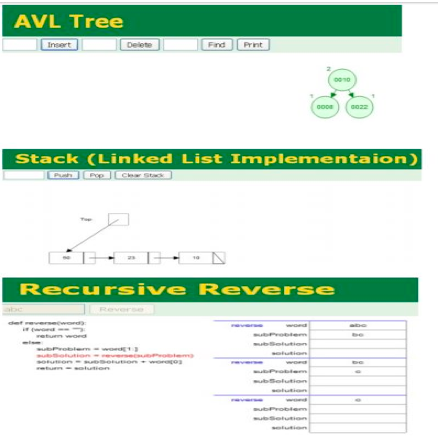
\includegraphics[width=1.0\textwidth]{./sample}\\[0.1in]






\section{Link To The Implementation}
Find our implementation using https://csceve17-005.000webhostapp.com
\paragraph{fig 2}

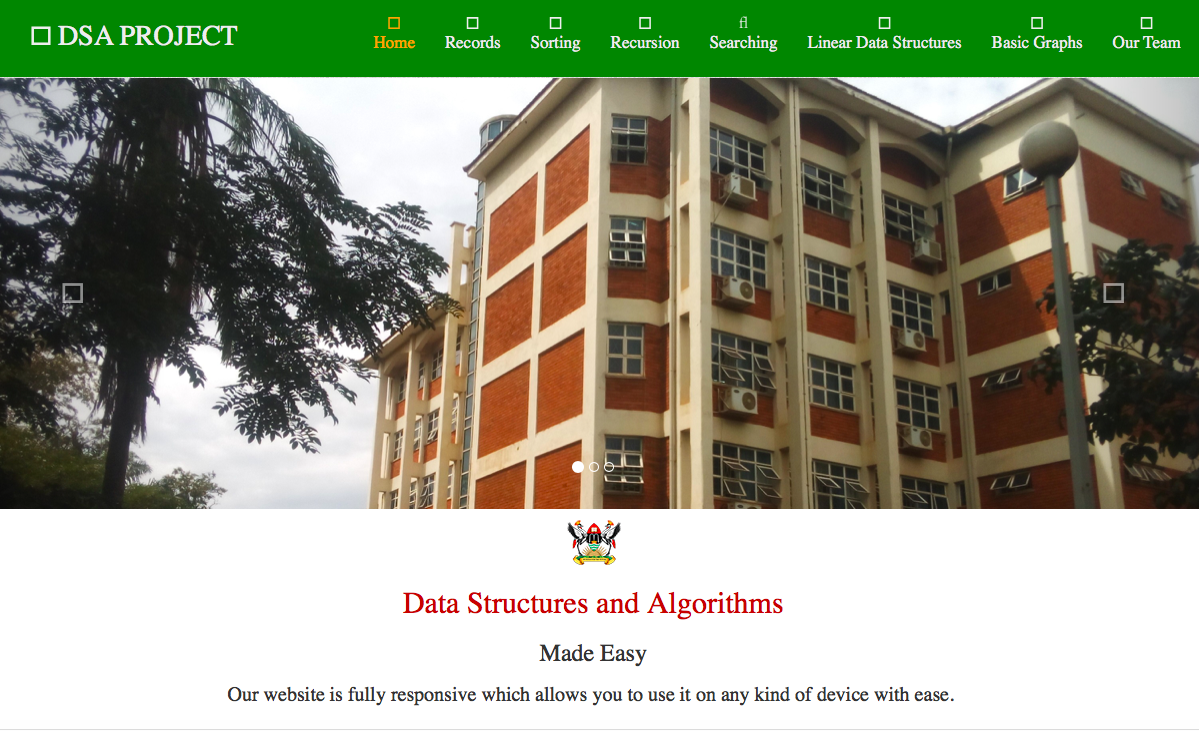
\includegraphics[width=1.0\textwidth]{./site}\\[0.1in]


\paragraph{fig 3}

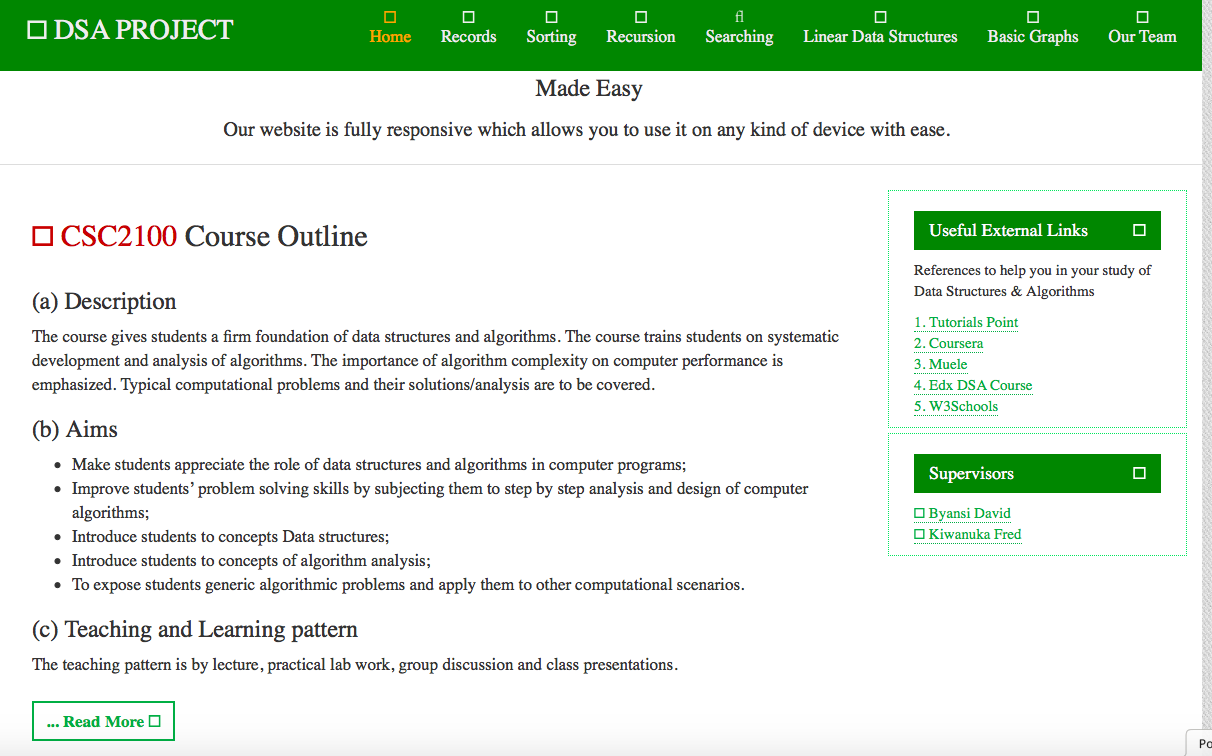
\includegraphics[width=1.0\textwidth]{./csoutline}\\[0.1in]

\paragraph{fig 4}

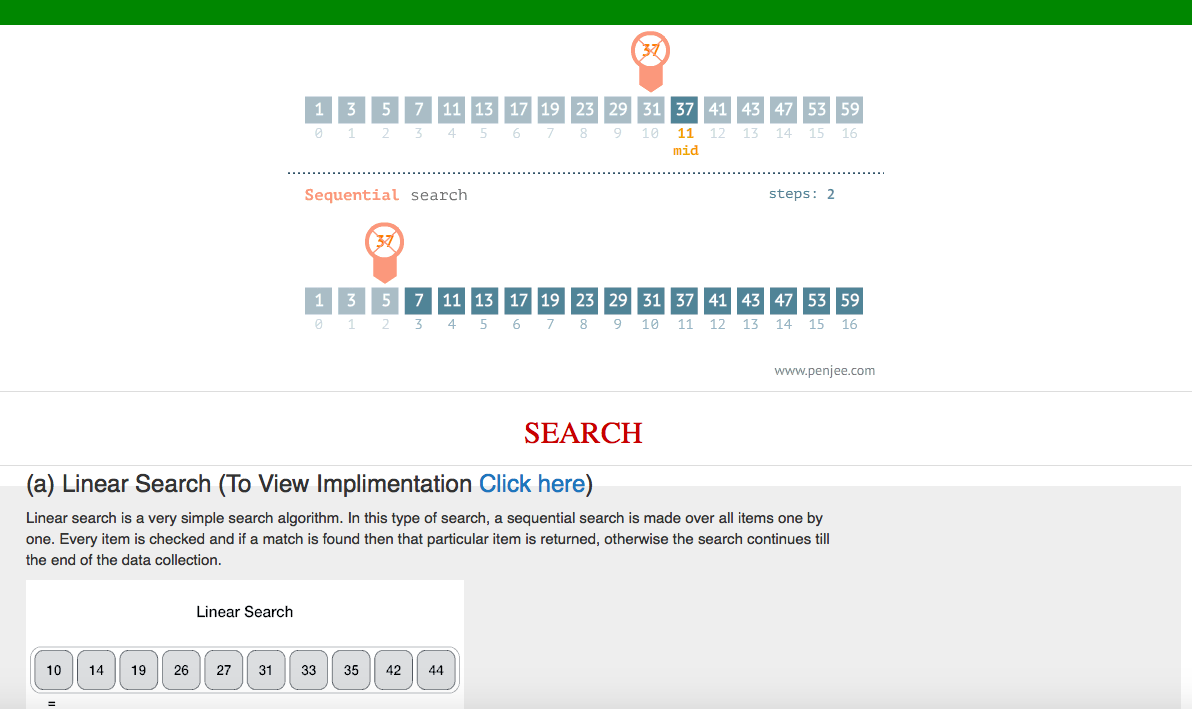
\includegraphics[width=1.0\textwidth]{./search}\\[0.1in]

\paragraph{fig 5}

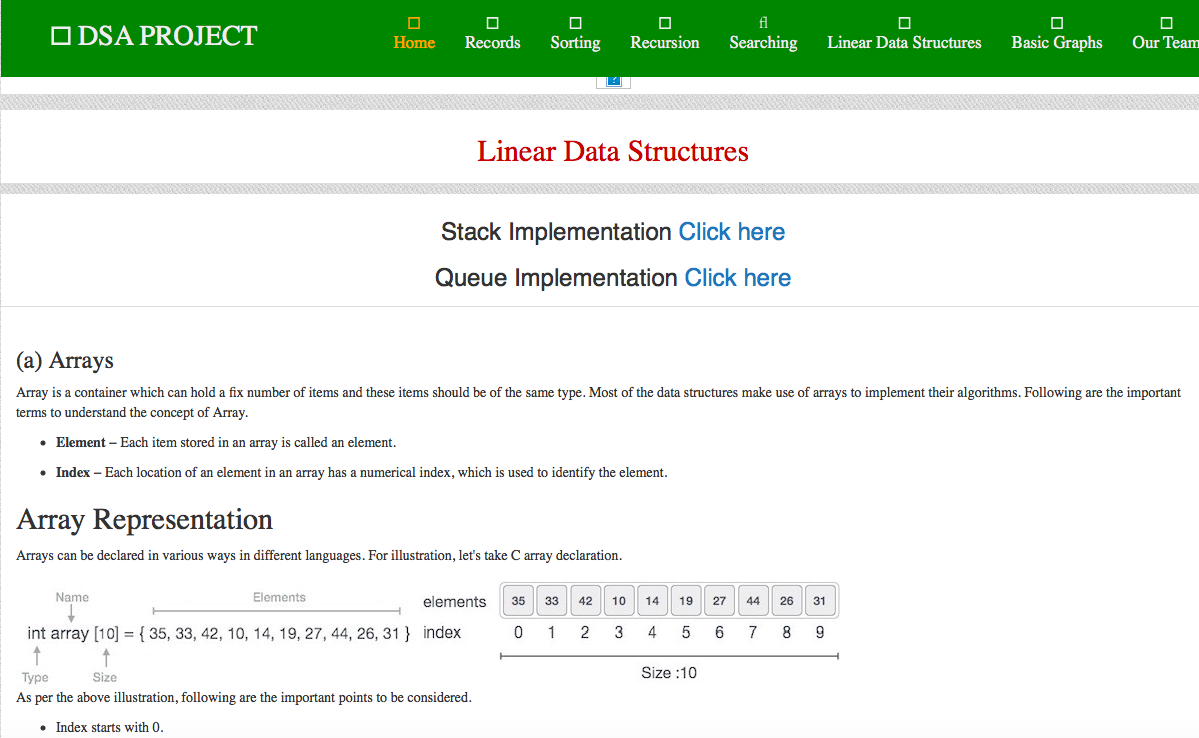
\includegraphics[width=1.0\textwidth]{./linear}\\[0.1in]

\paragraph{fig 6}

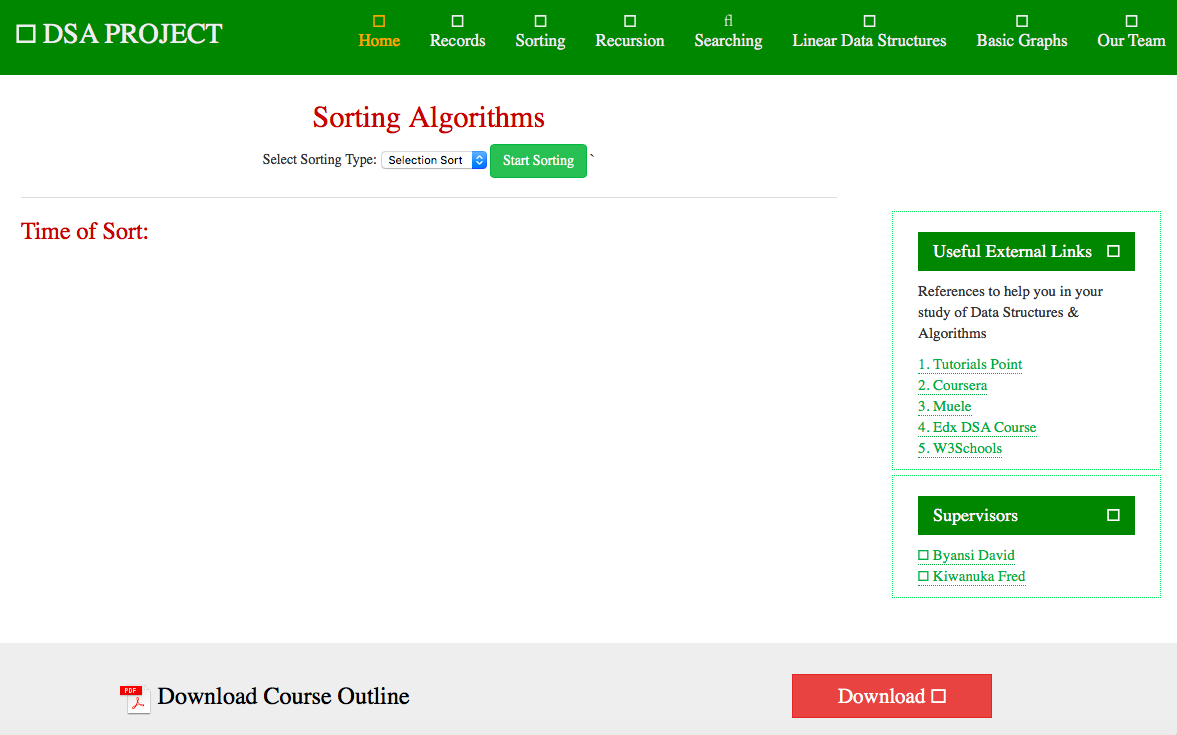
\includegraphics[width=1.0\textwidth]{./sort}\\[0.1in]

\paragraph{fig 7}

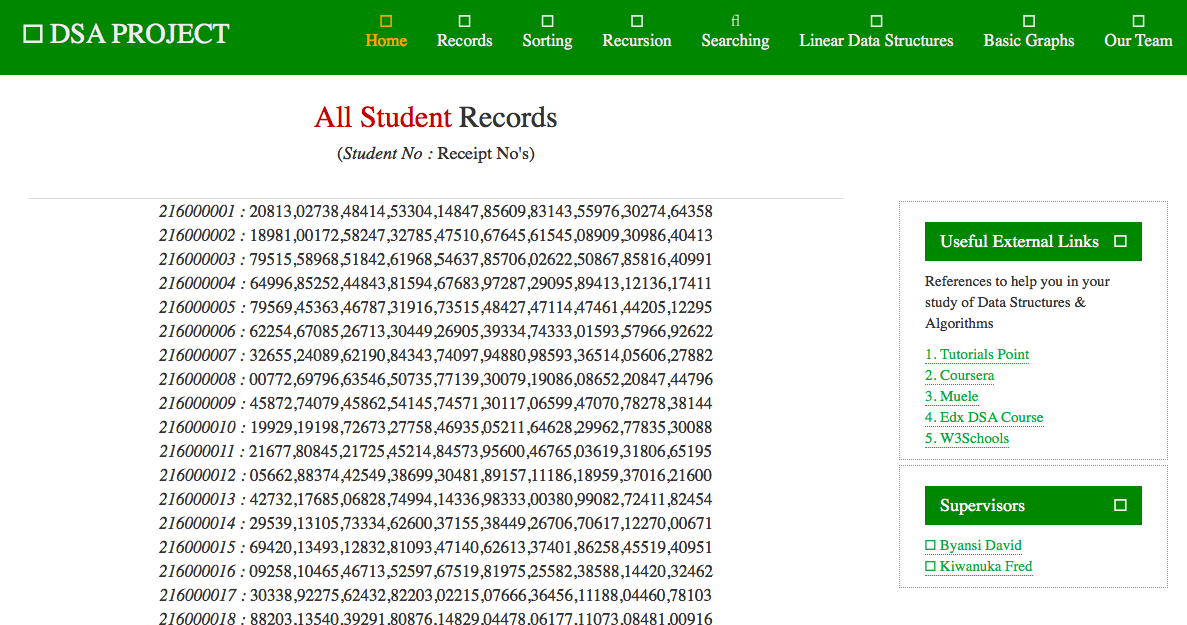
\includegraphics[width=1.0\textwidth]{./record}\\[0.1in]

\paragraph{fig 8}

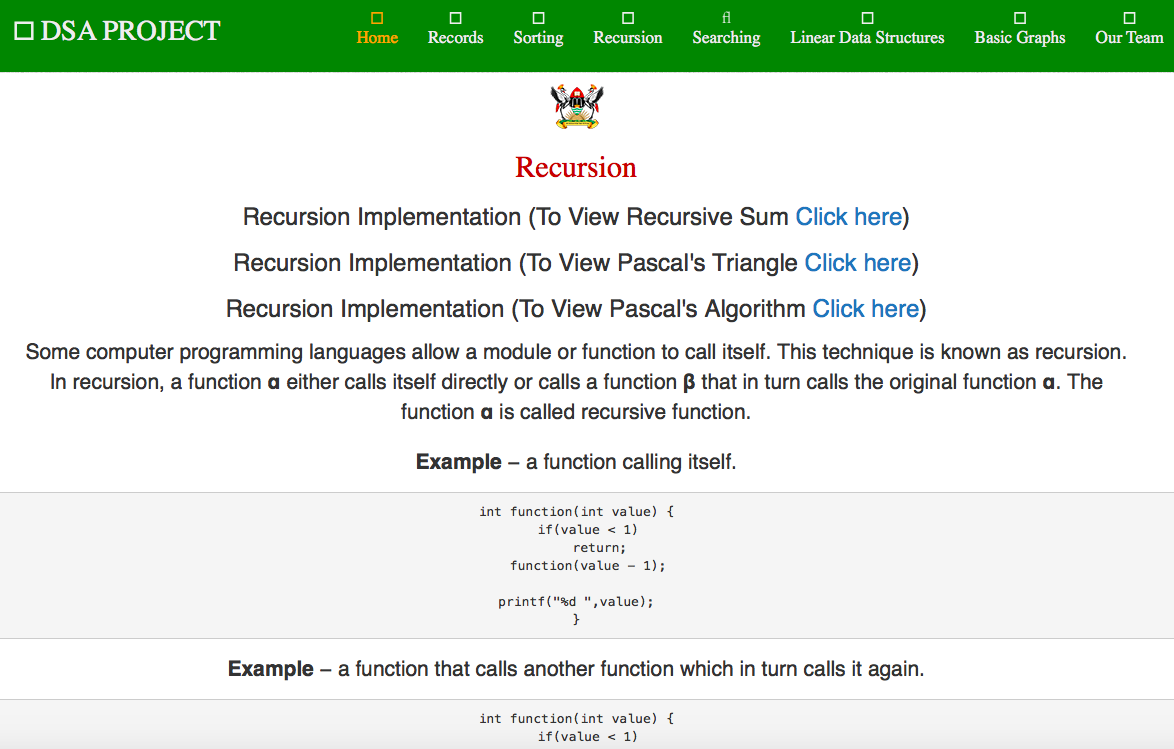
\includegraphics[width=1.0\textwidth]{./recursion}\\[0.1in]





\section{Conclusion}  
\paragraph{There are many factors which can influence the success of learning objects as support for student learning in university settings. Students will often need to be motivated and encouraged to use the independent learning resources. Also, it is unclear as to what forms of learning support best facilitate their use. }

\paragraph{\cite{de2006can}However, it is clear from the papers considered in this review that when designing tutoring systems, interaction with the system is the most important thing to consider for engaging students in the learning process. These interactions include: the use of multimedia like text supported with aural instructions, animations like the maze representation used in the Vedya tool, and tutorial videos for familiarization with the system.}

\paragraph{Making introductory data structures courses interesting and challenging requires projects that motivate students to enhance their programming abilities using the new data structures. This paper has discussed how a project involving competitive gaming motivates students to learn advanced game intelligence programming and improves their opinion of the course overall. The use of competition during an assignment can be used in any course where a suitable project can be developed. The competition server architecture can be used to enable the competitive environment. The major contribution is that interactive competition during the assignment increases student effort and satisfaction compared with projects where the competition comes after the assignment is completed.}
\paragraph{In this paper, we present a visualization tool designed to aid second-year computer science students learn Data Structures and Algorithms.}
\paragraph{This tool not only lets students visualize the commonly used data structures, but also allows students to  observe the execution of the algorithms. We believe this tool will be an effective supplement to traditional instruction. Because of the time limitation, only the most commonly used data structures are implemented in this version of the software package, which include arrays, stacks, queues, binary search tree, binary heap and priority queue.} 
\paragraph{\cite{kreutz2015software}This approach will allow users to use their own observable data structures, hence add more flexibility to the software. Another possible future enhancement for the software is to highlight the executing command line of the algorithm. This would help the user to better follow the execution of the algorithm.}
 

\newpage
\bibliographystyle{IEEEtran}
\bibliography{Reference}

\end{document}